\chapter{La transition énergétique est-elle favorable aux branches à fort contenu en emploi? Une analyse input-output pour la France} \label{chap:TE_Emploi}

\section{Introduction}
Dans la sphère académique, les politiques énergétiques, comme toutes les politiques sectorielles, sont principalement évaluées selon un critère coût-bénéfice ou coût-efficacité, ou encore en fonction de leur impact estimé sur le PIB, vu comme une approximation du bien-être économique. Leur impact sur l’emploi fait l’objet de moins d’analyses, comme le montre une simple consultation de la base de données académiques Web of Science : une interrogation à l’aide de la combinaison de mots-clés « energy AND (cost OR GDP OR welfare) » amène 96 549 résultats, soit 21 fois plus qu’une interrogation sur « energy AND (employment OR jobs) » (4 593 résultats). Dans le débat public français, en revanche, l’impact sur l’emploi de ces politiques a une importance équivalente à celle des analyses en termes de coût, de bien-être économique ou de PIB, comme le montre une interrogation de la base de données d’articles de presse Factiva : les mots-clés « transition énergétique AND (PIB OR coût) » renvoient 878 résultats, contre 895 pour « transition énergétique AND (emploi OR chômage) »\footnote{Interrogations effectuées le 23 septembre 2015}.

L’intérêt de prendre en compte l’emploi, plutôt que se focaliser sur le coût ou le surplus du consommateur, est double. Politiquement, de nombreux choix sont étudiés à l’aune de leur effet, réel ou supposé, sur l’emploi, donc une politique environnementale mauvaise pour l’emploi risque de ne jamais voir le jour. Par ailleurs, l’emploi présente une valeur au-delà du seul salaire \citep{Clark2015} qui renforce l’importance de cet indicateur.

Certes, les chercheurs en économie n’ont pas complètement négligé l’impact sur l’emploi de ces politiques. En particulier, une partie (minoritaire) du débat théorique sur le double dividende, initié par \citet{Pearce1991} et \citet{Goulder1994} porte sur l’emploi. \citet{Bosquet2000}, \citet{Chiroleu-Assouline2001} et \citet{Patuelli2005} proposent des revues de littérature. On peut noter l’absence de consensus dans ces travaux, avec des résultats très divers selon les hypothèses retenues. 

Avec l’essor des préoccupations liées aux changements climatiques, une attention nouvelle s’est portée sur la question des emplois liés à la transition énergétique, et en particulier aux énergies renouvelables. De nombreuses études technico-économiques comparent différentes techniques de production d’énergie (et/ou d’économie d’énergie). Plusieurs systèmes de mesure coexistent dans la littérature. Un premier est le nombre d’emploi par capacité installée, en kW. \citet{Cameron2015} passent en revue 70 études de ce type. Un autre système de mesure est le nombre d’emplois par énergie produite, en kWh. \citet{Wei2010} synthétisent ces études pour les Etats-Unis. Cependant, ces deux mesures présentent un biais en faveur des options techniques et organisationnelles les plus coûteuses : si une option coûte dix fois plus cher qu'une autre pour installer un kW ou produire un kWh, il est très probable qu'elle crée plus d'emplois par kW ou kWh, car la rémunération du travail represente environ deux tiers de la valeur ajoutée \citep{Cotis2009}. Or, des agents économiques (ménages, entreprises, administrations publiques…) vont nécessairement payer pour ce surcoût et vont par conséquent réduire d'autres consommations, d’où des destructions d’emplois ignorées par ce ratio. Pour cette raison, dans la présente étude nous calculons le ratio emplois par euro de demande finale.

Par ailleurs, plusieurs études menées à l’aide de modèles macroéconomiques ont étudié l’effet sur le PIB mais aussi sur l’emploi de politiques climatiques, principalement de taxes sur les émissions de CO\textsubscript{2}. On peut citer notamment les travaux de \citet{Lehr2008}, \citet{Lehr2012} ou encore \citet{EY2015} pour le compte de l’ADEME. En France, le modèle macroéconomique Three-ME, développé par l’ADEME et l’OFCE, a été utilisé pour quantifier le scénario « visions énergétiques 2030-2050 » de l’ADEME. Il aboutit à +330 000 emplois en 2030 et +825 000 en 2050, par rapport à un scénario tendanciel \citep{ADEME2013}. Ces travaux sont utiles, mais leurs résultats sont très dépendants de diverses hypothèses qui, du fait de la complexité de ces modèles, sont peu compréhensibles hors de la communauté des modélisateurs. Ainsi, deux modèles macroéconomiques ont été utilisés pour évaluer le paquet « climat-énergie » de la Commission européenne : E3ME, de Cambridge Econometrics, et GEM-E3, de la National Technical University of Athens. Les résultats du premier modèle en termes de PIB et d’emploi sont beaucoup plus favorables, pour des raisons qu’il est difficile de saisir, au-delà d’affirmations assez générales comme l’opposition entre le caractère néokeynésien du premier et néoclassique du second \citep{Bruyn2014}.

De nombreuses autres études portant sur l'emploi utilisent des modèles input-output simples. On les retrouve dans des sujets aussi divers que les programmes d'efficacité énergétique dans le bâtiment \citep{Scott2008}, la biodiversité \citep{DeBeir2015}, le chauffage par biomasse \citep{Madlener2007}, les biocarburants \citep{Neuwahl2008} ou encore des études plus générales sur la transition énergétique \citep{Quirion2013}. 
Les mécanismes à l’œuvre dans ces travaux sont plus faciles à comprendre car c’est alors la différence de contenu en emploi (au sens du ratio du nombre d'emplois par euro de demande finale) entre les branches en progression et celles en régression qui détermine l’effet net sur l’emploi. Cependant, ces études n’expliquent pas l’origine des écarts de contenu en emploi entre les branches : si un contenu en emploi plus élevé dans une branche provient, par exemple, de salaires plus faibles ou de moins d’importations. 
Pourtant, la différence est importante : dans un cas, il s’agit de relocaliser des emplois ; dans l’autre, de favoriser des créations d’emplois moins rémunérés.

Dans cet article, nous ne cherchons pas à calculer l’effet sur l’emploi d’un scénario ou d’une politique de transition énergétique mais à estimer le contenu en emploi et en gaz à effet de serre des différentes branches de l’économie française, ainsi qu’à décomposer les écarts de contenu en emploi selon une série de facteurs explicatifs. Cette approche descriptive permet d’apporter un éclairage qualitatif sur quelques substitutions interbranches impliquées par la transition énergétique. Par « transition énergétique », dans tout l’article nous ne faisons pas référence à un scénario particulier, mais à une évolution vers une sortie des énergies fossiles, nécessaire pour respecter l’objectif d’une division par quatre des émissions de gaz à effet de serre en France d’ici 2050, objectif fixé dans la loi depuis 2005\footnote{Loi de programme fixant les orientations de la politique énergétique (POPE) du 13 juillet 2005}.

En termes de méthode, cet article se rapproche des études de balance en emploi, qui mobilisent également les outils d’analyse entrées-sorties afin d’évaluer l’effet des échanges internationaux sur l’emploi. Ces analyses permettent une description fine distinguant les types de branches qui contribuent aux déséquilibres, les catégories de travailleurs touchés, etc. \citep{Guimbert2002}. La même méthodologie est d’ailleurs appliquée pour étudier l’empreinte carbone de la demande finale, afin de comptabiliser les émissions directes et indirectes \citep{Xu2014, Lenglart2010}. Cette analyse est notamment appliquée à l’étude des échanges commerciaux \citep{Dong2010}.

Le même cadre comptable peut être appliqué de façon dynamique, pour voir l’évolution du nombre d’emplois en faisant apparaitre les contributions des grands facteurs explicatifs. \citet{Barlet2009} observent les contributions respectives de la productivité, de la demande intérieure, des importations et des exportations. Cette dernière méthodologie est également de plus en plus utilisée pour comprendre les évolutions des émissions de gaz à effet de serre \citep{Martin2014a}.

Notre approche s’inscrit à l’intersection de ces deux démarches. Nous utilisons le même cadre comptable, et une décomposition proche de celle de \citet{Barlet2009} mais nous nous inscrivons dans un cadre statique, à l’instar des études de balance en emploi. L’originalité de notre article est de comparer le contenu en emploi de chaque branche à la moyenne de l’économie nationale et de décomposer cet écart pour chacune des branches selon quelques facteurs explicatifs. Plutôt que d’observer l’évolution temporelle de chaque branche, nous comparons les branches à la moyenne de l’économie et, grâce à ce point de repère, les unes par rapport aux autres. 

De plus, nous calculons dans un même cadre le contenu en emploi et le contenu en émissions de gaz à effet de serre sur le territoire. Notre approche permet de visualiser quelles branches permettent de créer de l’emploi en France tout en réduisant les émissions pour respecter les engagements internationaux de la France ; mais elle n’indique pas les emplois créés hors de France, ni une empreinte carbone incluant les émissions associées aux importations et aux exportations \citep{Pasquier2012}.

La méthode entrées-sorties s'appuie sur quelques hypothèses bien connues. Une hypothèse d’homogénéité des produits d’une branche est nécessaire pour notre décomposition du contenu en emploi et pour la description statique de l’économie. Etudier les effets d’une variation de la demande finale implique d’adopter deux autres hypothèses : une hypothèse de rendements constants (la consommation additionnelle ne modifie pas le système productif et le progrès technique n'est pas inclus) et une hypothèse que les effets induits autre que ceux capturés par la matrice de Leontief sont négligeables \citep{Freyssinet1977}. Ces hypothèses doivent amener à être prudent sur l’interprétation des résultats, et impliquent de ne considérer ni des variations trop importantes de la demande, ni un horizon temporel trop lointain.
Sous réserve de ces hypothèses supplémentaires, notre approche descriptive pourra être utilisée de façon plus normative, dans le but de guider l’action publique en donnant une idée des effets de premier ordre liés à une réallocation de la demande finale.

Le plan retenu est le suivant : nous présentons la méthode et les données utilisées dans la partie  \ref{sec:methode_donnees}, les résultats dans la partie \ref{sec:resultats}, puis nous concluons.


\section{Méthode et données}
\label{sec:methode_donnees}

\subsection{Données}
Nous utilisons trois sources de données, toutes publiées par Eurostat et concernant la France en 2010. Elles utilisent la nomenclature NACE rév. 2 en 64 branches.
\begin{itemize}
	\item Premièrement, le tableau entrées-sorties (TES) pour la France, au niveau de désagrégation A64, pour l’année 2010, à prix courant, préparé par l’Insee et publié par Eurostat (code Eurostat \href{http://appsso.eurostat.ec.europa.eu/nui/show.do?dataset=naio_cp18_r2&lang=en}{naio\_cp18\_r2}). Nous utilisons les tableaux fournis par Eurostat et non par l’INSEE pour trois raisons : la désagrégation est supérieure, avec 64 niveaux contre 38 pour les TES actuellement publiés par l’Insee (le TES à 118 branches n’est plus publié par l’Insee depuis 2007) ; l’utilisation des données Eurostat permet d’appliquer à notre analyse à tout pays européen ou à l’UE ; et ce TES distingue les consommations intermédiaires importées de celles produites en France, ce qui est indispensable pour calculer le contenu en emploi. Nous utilisons le tableau à prix courants car nous ne cherchons pas à étudier une évolution, mais la structure de l’économie pour une année donnée.
	\item Deuxièmement, l’emploi en équivalent temps plein (ETP), code Eurostat \href{http://appsso.eurostat.ec.europa.eu/nui/show.do?dataset=nama_nace64_e&lang=en}{nama\_nace64\_e}. Ces données fournissent le détail entre emploi salarié et emploi non-salarié. 
	\item Troisièmement, les comptes physiques d’émissions ventilés par branche économique pour la France, préparés par le Citepa et le SOeS et diffusés par Eurostat. Les gaz à effet de serre inclus sont ceux couverts par le Protocole de Kyoto : CO\textsubscript{2}, CH\textsubscript{4}, N\textsubscript{2}O, PFC, HFC et SF\textsubscript{6} (code Eurostat \href{http://appsso.eurostat.ec.europa.eu/nui/show.do?dataset=env_ac_ainah_r2&lang=en}{env\_ac\_ainah\_r2}). Nous les agrégeons en tonnes équivalent-CO\textsubscript{2} en utilisant les potentiels de réchauffement global utilisés par le protocole de Kyoto (21 pour le CH\textsubscript{4}, 310 pour le N\textsubscript{2}O). 
\end{itemize} 
Enfin, nous corrigeons le TES afin d’inclure les revenus non-salariés du travail dans les compensations. L'emploi non-salarié recouvre les employeurs, les personnes établies à leur compte, les membres des coopératives de production et les travailleurs familiaux non rémunérés. Nous utilisons les données d'Eurostat sur le nombre d'ETP non-salariés, et nous le traduisons en revenus salariés équivalents en supposant un même revenu par ETP pour salariés et non-salariés. Nous le faisons afin de tenir compte des nombreux travailleurs non-salariés, notamment dans la branche agriculture.

\subsection{Définition du contenu en emploi}
Suivant en cela une longue tradition \citep{Freyssinet1977, Husson1994}, nous définissons le contenu en emploi comme le nombre d’emplois (plus précisément d’ETP) localisés en France, nécessaires à la production générée par un million d’euros de demande finale adressé à une branche donnée et pour une année donnée. Ce nombre d’emplois comprend des emplois directs (c’est-à-dire dans la branche à laquelle s’adresse cette demande finale) et indirects (dans les branches en amont de cette dernière). Ainsi défini, le contenu en emploi correspond au terme de multiplicateur d’emploi qui existe également dans la littérature \citep{Miller2009}.

Nous choisissons donc de définir le contenu en ETP d’une branche i par :
\begin{equation}
ce_i= \frac{\text{Nombre d'ETP directs et indirects dus à l'activité de la branche i}}{\text{Millions d'euros de demande finale adressée à la branche i}}
\label{definition_ce}
\end{equation}
Cette méthode est préférable aux ratios emplois/chiffre d’affaire ou emplois/valeur ajoutée : le premier présente un biais au détriment des branches utilisant une forte proportion de consommations intermédiaires, donc d’emplois indirects, tandis que le second est imprécis car il ne distingue pas deux branches ayant le même ratio emplois/VA mais adressant leurs demandes de consommations intermédiaires à des branches présentant elles-mêmes un contenu en emploi différent, donc générant au total un nombre différent d’emplois.

\subsection{Calcul du contenu en emploi}
L’utilisation des tableaux entrées-sorties (TES) de la comptabilité nationale permet de calculer le contenu en emploi pour les différentes branches de l’économie, en nous appuyant sur la méthode de \citet{Leontief1986}. Le point de départ de cette méthodologie est l’équilibre comptable entre ressources et emplois pour les produits de chaque branche, pour une année donnée. Les données permettent en outre de distinguer un équilibre correspondant au territoire national (i.e. la part intérieure), représenté dans l'équation \ref{equilibre_interieur}, et un équilibre pour les importations, dans l'équation \ref{equilibre_imports} :
\begin{equation}
\pmb{p^d} = \pmb{CI^d} \cdot \pmb{i} + \pmb{d^d}	
\label{equilibre_interieur}
\end{equation}
\begin{equation}
\pmb{m} = \pmb{CI^m} \cdot \pmb{i} + \pmb{d^m}	
\label{equilibre_imports}
\end{equation}
où l'exposant \textit{d} fait référence à une part intérieure (ou domestique) et l'exposant \textit{m} à une part importée. $\pmb{p^d}$ indique la production intérieure, $\pmb{CI^d}$ et $\pmb{CI^m}$ sont les matrices des consommations intermédiaires intérieures et importées, $\pmb{d^d}$ et $\pmb{d^m}$ les demandes finales intérieures et importées et $\pmb{m}$ les importations de biens finaux. $\pmb{i}$ est le vecteur colonne composé uniquement de 1. Les notations suivent les conventions suivantes : les lettres en gras et minuscules d’imprimerie indiquent un vecteur-colonne, les capitales d’imprimerie en gras une matrice carrée. Enfin, on réserve l'exposant \textit{t} pour les valeurs totales, somme des valeurs intérieures et importées. Ainsi, la demande finale totale $\pmb{d^t=d^d+d^m}$ et l'ensemble des consommations intermédiaires vaut $\pmb{CI^t=CI^d+CI^m}$.


On peut introduire les matrices des coefficients techniques $A^d$ et $A^m$, c'est-à-dire les matrices telles que :
\begin{equation*}
A^d = (A^d_{ij}) = \left( \frac{CI^d_{ij}}{P_j} \right) \quad \text{et} \quad A^m = (A^m_{ij}) = \left( \frac{CI^m_{ij}}{P_j} \right)
\end{equation*}
En utilisant ces matrices de coefficients techniques, on peut réarranger les équations \ref{equilibre_interieur} et \ref{equilibre_imports} afin d'obtenir une relation liant directement la production à la demande finale :
\begin{equation}
\pmb{p^d} = (\pmb{I} - \pmb{A^d})^{-1} \cdot \pmb{d^d}	
\label{equilibre_interieur2}
\end{equation}
où $\pmb{I}$ est la matrice identité. La matrice $(\pmb{I} - \pmb{A^d})^{-1}$ est la matrice inverse de Leontief. 
Elle indique la production directe et indirecte nécessaire pour satisfaire une demande intérieure. 
Plus précisément, le terme d'indices (i,j) de cette matrice $(\pmb{I} - \pmb{A^d})^{-1}$ donne la production dans la branche $i$ engendrée par unité de demande finale adressée à la branche $j$.

L'équation \ref{equilibre_interieur2} donne la somme de la production dans chaque branche générée par le vecteur de demande finale. On peut cependant affiner cette formule afin d'extraire plus d'information. Pour cela, on introduit l'opérateur $\widehat{  }$ qui transforme un vecteur colonne en matrice carrée diagonale. L'équation \ref{equilibre_interieur2} devient :
\begin{equation}
\pmb{P^d} = (\pmb{I} - \pmb{A^d})^{-1} \cdot \widehat{\pmb{d^d}}	
\label{equilibre_interieur3}
\end{equation}
Dans cette nouvelle version, on obtient une matrice carrée $\pmb{P^d}$ pour la production intérieure. Le terme d'indice (i,j) de cette matrice indique la production générée dans la branche $i$ du fait de la demande adressée à la branche $j$.

Enfin, on peut lier la production à la demande totale, et non à la seule demande intérieure. Cet ajout permet de voir l'impact des importations finales. On suppose que le taux $MF_i = \frac{D^d_i}{D^t_i}$ de demande intérieure dans la demande finale totale $\pmb{d^t}$ est constant pour chaque branche $i$ - autrement dit, on suppose que le taux d'importations finales dans la demande finale totale, $1 - MF_i$, est constant pour chaque branche. De façon matricielle, on peut l'écrire $\pmb{d^d} =~\widehat{\pmb{mf}} \cdot~\pmb{d^t}$, avec $\pmb{mf}$ le vecteur colonne des taux d'importations. Alors, l'équation \ref{equilibre_interieur3} devient :
\begin{equation}
\pmb{P^d} = (\pmb{I} - \pmb{A^d})^{-1} \cdot \widehat{\pmb{mf}} \cdot \widehat{\pmb{d^t}}	
\label{equilibre_interieur4}
\end{equation}

Maintenant, si l'on connait le nombre d'ETP $ETP_j$ dans chaque branche $j$, et que l'on admet que ce nombre d'emplois est proportionnel à la quantité $P_j$ produite, alors on peut définir la matrice colonne du nombre d'emplois par unité de production : 
$$\pmb{e} = (e_j) = ( \frac{ETP_j}{P_j})$$

Le lien entre le nombre d'emplois et la demande finale se déduit alors de \ref{equilibre_interieur4} :
\begin{equation}
\pmb{etp} =~\widehat{\pmb{d^t}} \cdot~\widehat{\pmb{mf}} \cdot~(\pmb{I} - (\pmb{A^d})^T)^{-1} \cdot \pmb{e}
\label{emploi}
\end{equation}
où $^T$ désigne l'opérateur de transposition matricielle.
Le contenu en emploi, défini dans l'équation \ref{definition_ce} comme le nombre d'emplois par unité de demande finale, découle de l'équation \ref{emploi} en posant une demande finale unitaire, autrement dit $\widehat{\pmb{d^t}}~= \pmb{I}$. On aboutit à la formule du contenu en emploi $\pmb{ce}$: 
\begin{equation}
\pmb{ce} = ~\widehat{\pmb{mf}} \cdot~(\pmb{I} - (\pmb{A^d})^T)^{-1} \cdot \pmb{e}
\label{contenu_emploi}
\end{equation}
où le terme $ce_i$ est le contenu en emploi de la branche $i$. C'est cette formule qui est utilisée pour calculer le contenu en emploi d'une branche.



\subsection{Décomposition du contenu en emploi}

Les calculs de contenu en ETP font apparaitre de fortes disparités entre les branches (cf. annexe \ref{app:tableau_ce}). Il est cependant utile de ne pas s’arrêter à la valeur du contenu en emploi, mais de détailler sa composition. Le contenu en emploi d’une branche peut en effet avoir une signification très différente s’il est faible du fait de salaires élevés ou d’importations importantes : dans le premier cas, déplacer la demande adressée à cette branche revient à réduire les salaires ; dans le second, à relocaliser la production (ces effets seront étudiés à l'aide de modèles macroéconomiques dans le chapitre \ref{chap:mechanisms}).  Une analyse détaillée du contenu en emploi est donc nécessaire dès lors que l’on souhaite utiliser cet indicateur.

Les données de la comptabilité nationale fournissent de nombreuses informations pour décomposer le contenu en emploi des différentes branches. La formule \ref{contenu_emploi} permet de déterminer directement le contenu en emploi, mais il est possible de faire apparaitre des ratios intermédiaires utiles à l'analyse.

Tout d'abord, on peut décomposer le terme $\pmb{e}$ donnant le nombre d'emplois par unité de production. Plutôt que de passer directement de l'emploi à la production, on va chercher à faire apparaitre l'importance des taxes dans la valeur ajoutée, la part des salaires par rapport aux revenus du capital, et le niveau de salaires.
Le second terme à décomposer est $(\pmb{I} - (\pmb{A^d})^T)^{-1}$, afin de faire apparaitre les importations intermédiaires. En effet, comme $\pmb{A^d} = \pmb{A^t} - \pmb{A^m}$, la production intérieure va dépendre à la fois des fonctions de production représentées dans $\pmb{A^t}$ et des taux d'importations reflétés par $\pmb{A^m}$.

\begin{equation}
\forall i \quad ce_i = \sum_j MF_i \cdot V_{ij} \cdot MI_{ij} \cdot T_j \cdot L_j \cdot N_j
\end{equation}
où
\begin{itemize}
	\item $MF_i $ est le taux de demande intérieure dans la demande finale totale ;
	\item $V_{ij}$ est la valeur ajoutée intérieure par unité de production ;
	\item $MI_{ij}$ indique le taux d'importations intermédiaires ;
	\item $T_j$ est le taux de taxes et subventions (« Autres impôts sur la production », code D29\_M\_D39 et « Impôts moins subventions sur les produits », code D21\_M\_D31) dans la valeur ajoutée augmentée des « Impôts moins subventions sur les produits »;
	\item $L_j$ représente la part des rémunérations du travail dans la valeur ajoutée moins les « autres impôts sur la production » (D29\_M\_D39) ;
	\item $N_j$ est égal à l’inverse du salaire. Il mesure donc le niveau des salaires.
\end{itemize}

Cette suite de ratio en cascade suit une logique de production illustrée par la figure \ref{fig:schema_decompo}.

\begin{figure}[!hb]
	\centering
	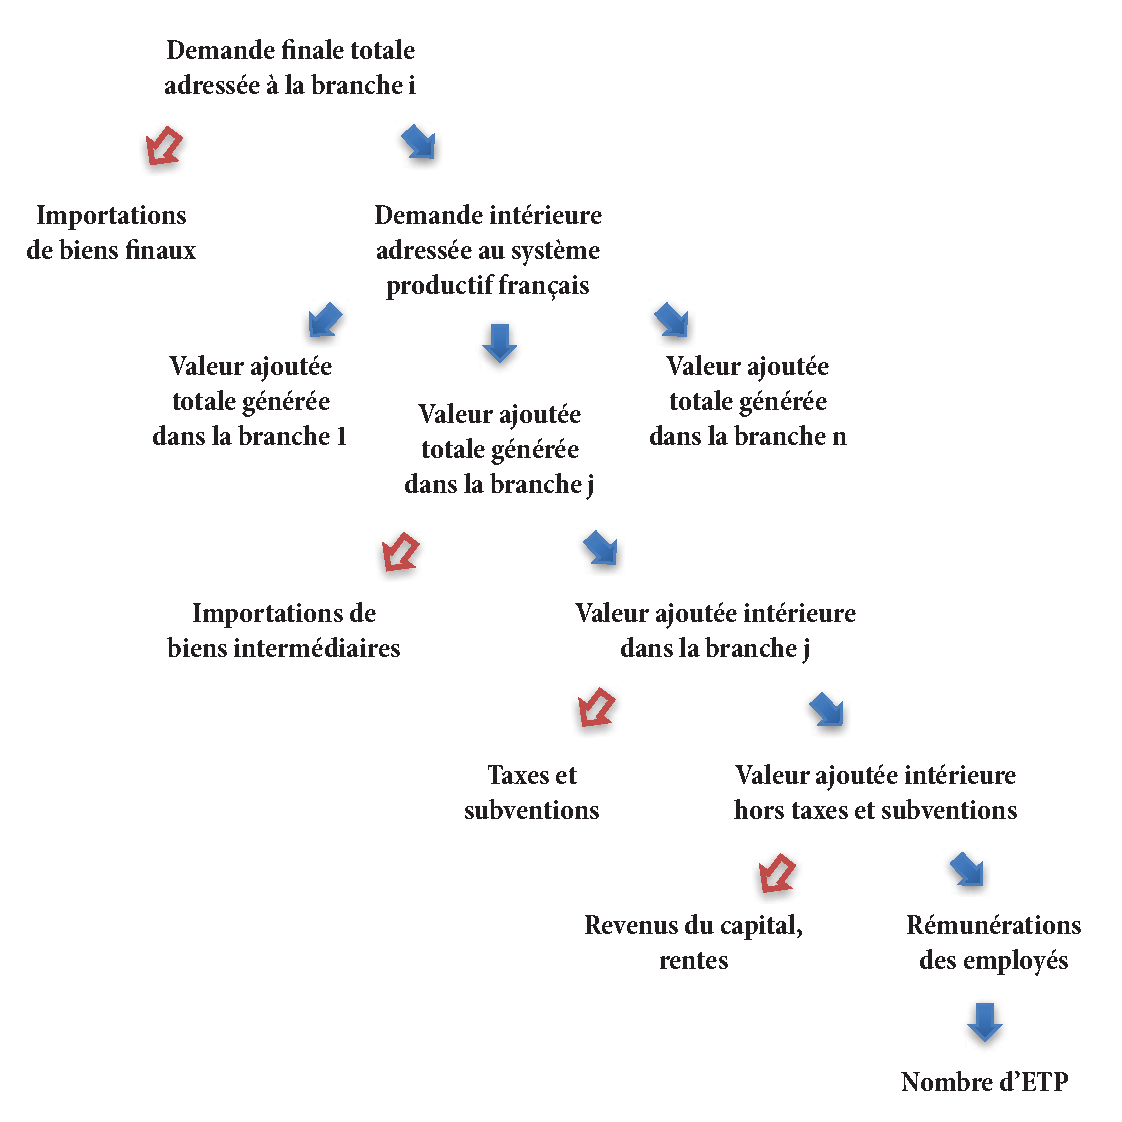
\includegraphics[height=12cm]{figures/Schema_decompo/schema_decompo.pdf}
	\caption{Schéma de décomposition du contenu en emploi. \\Source : Auteurs}
	\label{fig:schema_decompo}
	\captionsetup{justification=raggedright}
	\caption*{Lecture : une demande finale totale va susciter d’une part des importations finales, et d’autre part une demande intérieure qui sera adressée à la production intérieure. La demande intérieure suscite une production dans d’autres branches du fait des consommations intermédiaires, et donc la création de valeur ajoutée dans plusieurs branches. Une partie de cette valeur ajoutée est captée à l’étranger à cause des importations de produits intermédiaires. Dans la valeur ajoutée intérieure restante, une partie sert à payer des taxes ou provient de subventions. Enfin, la valeur ajoutée hors taxes et subventions rémunère le capital et les compensations salariales. Ces dernières servent à employer des travailleurs.}
\end{figure}

\subsection{Comparaison à la moyenne et décomposition LMDI}
Pour toute branche $i$, on peut comparer le contenu en emploi de cette branche avec la moyenne de l’économie nationale – cette moyenne nationale étant définie via des ratios moyens (la définition précise est donnée en annexe \ref{app:def_moyenne}).
\begin{equation}
ce_i - ce_{i,m} = \sum_j MF_i \cdot V_{ij} \cdot MI_{ij} \cdot T_j \cdot L_j \cdot N_j - \sum_j MF_m \cdot V_{ij,m} \cdot M_{ij,m} \cdot T_m \cdot L_m \cdot N_m
\end{equation}
En remarquant que les coefficients $V_{ij}$ jouent le rôle de clé de ventilation, et en utilisant la méthode LMDI (Logarithm Mean Divisia Index) de décomposition d’indice développée par \citet{Ang2005}, on peut transformer cette différence en somme de termes traduisant l’apport de chaque facteur (les détails sont donnés en annexes \ref{app:ventilation_LMDI} et \ref{app:decompo_LMDI}) :
\begin{equation}
ce_i - ce_{i,m} = \Delta MF_i + \Delta MI_i + \Delta T_i +\Delta L_i + \Delta N_i
\end{equation}
Il est ainsi possible de déterminer l’impact des différents facteurs dans la composition et le niveau du contenu en ETP. On peut donc répondre à la question : pourquoi le contenu en emploi d’une branche est-il élevé ? Est-ce du fait d’importations finales ou intermédiaires faibles, de taxes faibles, d’une forte part du travail dans la valeur ajoutée, ou de salaires bas ?


\subsection{Contenu en gaz à effet de serre}
Le contenu en émissions de gaz à effet de serre est calculé avec la même méthode que pour le contenu en emploi. A partir des émissions de gaz à effet de serre par branche, on construit le vecteur $\pmb{g}$ donnant le ratio des émissions de gaz à effet de serre (GES) par unité de production. Alors, le contenu en émissions directes et indirectes $\pmb{cg}$ est donné par la relation :
\begin{equation}
\pmb{cg} =~\widehat{\pmb{mf}} \cdot~(\pmb{I} - (\pmb{A^d})^T)^{-1} \cdot \pmb{g}
\end{equation}
Il convient de noter que notre approche traite les émissions du point de vue de la production, c’est-à-dire aux émissions sur le territoire. Notamment, nous n’intégrons pas les émissions associées aux importations. Ce choix permet d’analyser les leviers utiles aux politiques publiques pour tenir leurs engagements nationaux ou européens. En revanche, une logique cherchant à attribuer les émissions aux consommateurs – par exemple avec la notion d’empreinte carbone - devrait également prendre en compte les émissions associées aux importations \citep{Pasquier2012}. En outre, en regardant les émissions par branche d’activité, nous omettons les émissions liées aux consommations finales, notamment dans les transports des ménages et le chauffage. 


\subsection{Branches pour lesquelles la méthode est inapplicable}
Nous appliquons la méthodologie en utilisant le tableau entrées-sorties d’Eurostat à 64 branches. Toutefois, notre méthodologie ne peut pas être appliquée à quatre branches de la nomenclature NACE Rév. 2 :
\begin{itemize}
	\item La branches B (« Industries extractives ») car la demande finale intérieure est négative en 2010, à cause des variations de stock. On ne peut donc pas prendre le logarithme de cette demande ;
	\item La branche K66 (« Activités auxiliaires de services financiers et d'assurance ») qui n’a aucune demande finale ni intérieure. Là encore, on ne peut pas prendre le logarithme ;
	\item La branche L68A (« Loyers imputés des logements occupés par leur propriétaire ») qui ne verse aucun salaire ;
	\item La branche T (« Activités des ménages en tant qu'employeurs ; activités indifférenciées des ménages en tant que producteurs de biens et services pour usage propre ») qui n’utilise aucune consommation intermédiaire. 
\end{itemize}

Par la suite, nous ignorons donc ces quatre branches, ce qui n’est pas gênant car trois de ces branches (43, 45, 64) constituent des branches particulières de l’économie, et la branche 4 présente une activité très réduite en France (inférieure à 0,13\% des ressources totales de l’économie).


\section{Résultats}
\label{sec:resultats}

\subsection{Principaux déterminants des différences de contenu en emploi}
Quels sont les grands déterminants permettant d’expliquer les différences de contenu en emploi entre les différentes branches économiques ? Pour répondre à cette question, il suffit de calculer, sur l’ensemble des branches considérées, l’écart-type de nos cinq facteurs explicatifs : plus celui-ci est élevé, plus ce facteur diffère d’une branche à l’autre et plus il explique une part importante des écarts de contenu en emploi entre les branches.

\begin{table}[!h]
	\centering
	\caption{Ecart-type des cinq facteurs explicatifs des écarts de contenu en emploi, 
		sur les 60 branches considérées. \\ 
		Source : calculs des auteurs à partir de données Eurostat.}
	\label{tab:ecart_type}
	\begin{tabular}{ll}
		\toprule
		Facteur explicatif & Ecart-type \\
		\midrule
		$\Delta N$ & 3,12 \\
		$\Delta L$ & 2,34 \\
		$\Delta MF$ & 1,67 \\
		$\Delta MI$ & 0,98 \\
		$\Delta T$ & 0,80 \\
		\bottomrule
	\end{tabular}
\end{table}


Comme l’indiquent les chiffres du tableau \ref{tab:ecart_type}, la principale cause de variation de contenu en ETP réside dans la différence de salaires, suivie de la part du travail dans la valeur ajoutée, puis, dans l’ordre, du taux d’importations de produits finaux et intermédiaires. Enfin, les taxes nettes des subventions jouent un rôle mineur dans l’explication des variations de contenu en emploi entre les différentes branches. Ce paramètre est notamment important dans la branche agriculture, du fait des subventions de la politique agricole commune.


\subsection{Contenu en emploi et en émissions de gaz à effet de serre}

Ayant obtenu le contenu en émissions de GES, nous pouvons le croiser sur un graphique avec le contenu en emploi sur la figure \ref{fig:ges_emploi}. En faisant apparaitre la moyenne de l’économie (les lignes horizontale et verticale), on peut distinguer quatre quadrants, selon nos deux critères que sont le contenu en emploi et le contenu en GES :
\begin{itemize}
	\item Le cadran en haut à droite regroupe les branches à fort contenu en emploi et en GES. La plupart de ces branches sont liées à l’alimentation. On voit ainsi que l’agriculture présente de loin le contenu en GES le plus élevé parmi les branches de l’économie française, du fait des émissions de protoxyde d’azote (N\textsubscript{2}O) et de méthane (CH\textsubscript{4}). De plus, l’industrie agroalimentaire et l’agriculture se classent en tête quant aux émissions de GES totales générées de façon directe et indirecte, émissions indiquées par la taille des cercles. La pêche, l’hébergement-restauration et les transports terrestres (fret et services de transport) figurent également dans ce cadran. 
	\item En haut à gauche se trouvent les branches fortement émettrices et générant peu d’emplois. Cela inclut l’industrie chimique, la production d’électricité, les transports aériens, la métallurgie, les activités de cokéfaction et raffinage, le traitement des eaux usées, la production de produits minéraux non métalliques (ciment, verre…), les transports par eau et l’industrie du papier.
	\item Le cadrant en bas à droite regroupe les branches ayant un contenu en emploi élevé et un contenu en émissions de GES faible. Ce groupe inclut la plupart des activités du secteur tertiaire, mais également quelques branches du secteur secondaire, notamment la construction.
	\item En bas à gauche se trouvent les branches peu créatrices d’emplois, mais également peu émettrices. Ce groupe inclut de nombreuses industries, notamment de fabrication (textile, bois, caoutchouc), de produits métalliques, informatiques ou d’équipements électriques ; mais également de nombreuses branches des services.
\end{itemize}

Sur la figure \ref{fig:ges_emploi}, nous avons indiqué en gris foncé les branches couvertes par le système communautaire d’échange de quotas d’émissions de GES (EU ETS ou SCEQE). Aujourd’hui, ce système concerne plus de 11 000 installations, et couvre presque 45\% des émissions de gaz à effet de serre de l’Union Européenne. Les branches économiques concernées sont notamment la production d’électricité, la fabrication de produits métalliques, le raffinage de produits pétroliers, la production de ciment, verre, chaux et céramique, d’acides et de produits chimiques, ainsi que le transport aérien pour les seuls vols intracommunautaires \citep{EuropeanUnion2013}.

S’il est logique que les branches couvertes par l'EU ETS se trouvent dans la partie haute de cette figure, du fait de leur fort contenu en GES, il est frappant de constater que toutes se trouvent également à gauche de celle-ci, témoignant de leur faible contenu en emploi. Ce faible contenu en emploi s'explique principalement du fait d'importations élevées et/ou d'une faible part des salaires dans la valeur ajoutée (cf. annexe \ref{app:EU_ETS}).
Plus généralement, le faible contenu en emploi de ces branches rejoint le débat sur la complémentarité de l’énergie au capital et au travail. Cette question a fait l’objet de controverses depuis les années 1970 (cf. les références citées par Solow, \citeyear{Solow1987}) jusqu’à aujourd’hui \citep{Dissou2015, Fiorito2016}. 
Tenter d’y répondre passe par des estimations économétriques qui sortent du cadre de cet article. Mais le faible contenu en emploi des branches les plus intensives en gaz à effet de serre fournit un premier éclairage : si les politiques climatiques entraînent une réduction d’activité de ces branches, l’effet agrégé sur l’emploi sera plus modéré que ce qu’indique la part de ces branches dans le PIB, indicateur largement utilisé, par exemple par \citet{Sato2015}

Les branches situées en haut à droite, bien que présentant également un fort contenu en GES, ne sont pas couvertes par des politiques climatiques significatives. Pour les transports terrestres, la redevance kilométrique poids lourds adoptée lors du Grenelle de l’environnement a été abandonnée, tandis l’agriculture et la pêche ne sont couvertes ni par l'EU ETS ni par la composante carbone des taxes sur l’énergie, qui croît progressivement depuis 2014 et dont la montée progressive jusqu’à 100 euros par tonne de CO\textsubscript{2} en 2030 a récemment été inscrite dans la Loi de transition énergétique pour la croissance verte\footnote{Loi n°2015-992 du 17 août 2015 relative à la transition énergétique pour la croissance verte}.

\begin{figure}[!ht]
	\centering
	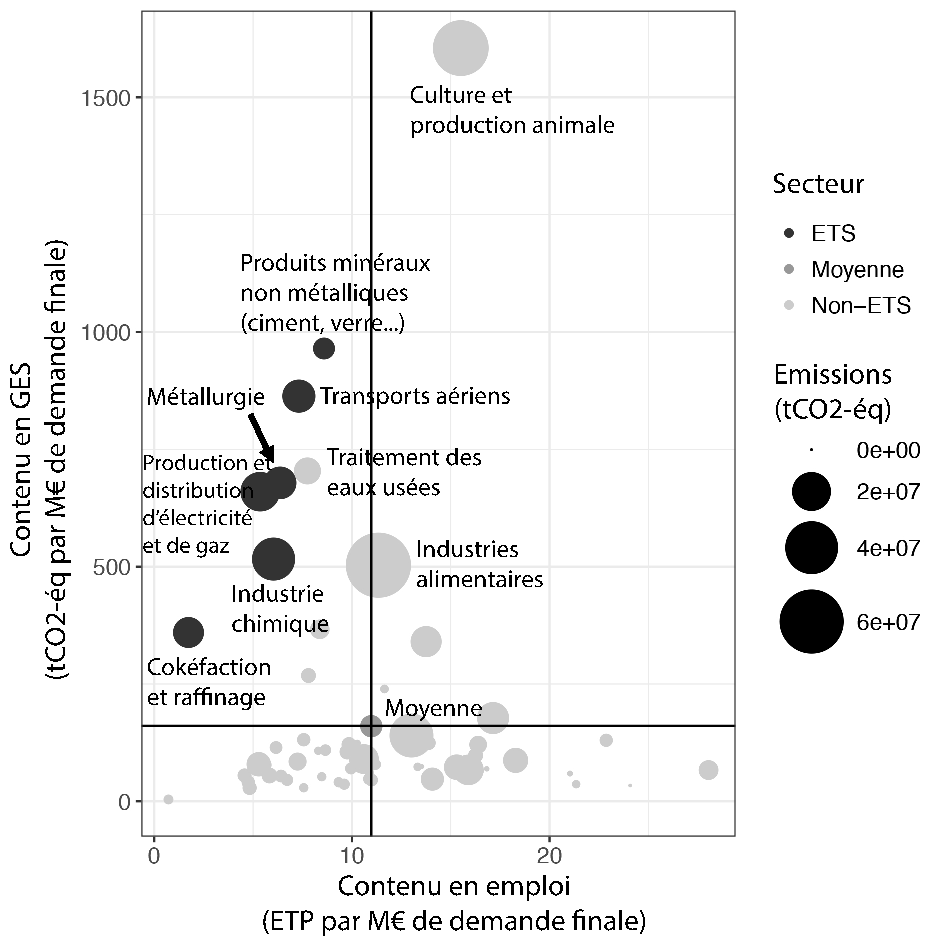
\includegraphics[height=11cm]{figures/GES_et_emplois/GES_emploi.pdf}
	\caption{Contenu en GES et en emploi des 64 branches de l'économie française. \\
		Sources : Calcul des auteurs à partir de données Eurostat.}
	\label{fig:ges_emploi}
	\captionsetup{justification=raggedright}
	\caption*{Lecture : la branche « Culture et production animale » de l’INSEE génère en moyenne 15,5 ETP et 1 600 tonnes d’équivalent-CO\textsubscript{2} par million d’euros de demande finale. La taille du cercle est proportionnelle à la quantité totale de gaz à effet de serre émise de façon directe et indirecte par la demande finale adressée à chaque branche. Le gris foncé indique les branches soumises à l’EU ETS.
		
		Les émissions directes des ménages, qui consistent essentiellement dans le transport terrestre privé et l’utilisation de gaz et de fioul pour le chauffage, l’eau chaude sanitaire et la cuisson, ne sont pas représentées ici car elles ne peuvent pas être analysées avec la même méthode. Une représentation incluant ces émissions est disponible dans l’annexe \ref{app:emissions_menages}. Les émissions considérées sont celles réalisées sur le territoire français, conformément aux engagements internationaux de la France ; les émissions liées aux importations ne sont pas incluses.}
\end{figure}

Les données publiées par Eurostat permettent d’effectuer le même croisement entre émissions et emploi, pour tout pays de l’Union Européenne. Ce travail a été réalisé pour l’Union européenne dans son ensemble, pour la même année (cf. annexe \ref{app:ges_emploi_EU}). On remarque une grande similitude avec les résultats pour la France, à part pour la branche électricité, gaz et vapeur, qui est beaucoup plus émettrice de GES au niveau européen qu'au niveau français, du fait de la forte part de nucléaire et d’hydraulique en France.


\subsection{Décomposition du contenu en emploi par branche}

\subsubsection{Remarques générales}

Le tableau \ref{tab:decompo_ce} montre le résultat de notre méthode pour les 60 branches de l’économie française (sur 64) auxquelles il est possible de l’appliquer. 
De façon générale, les branches industrielles présentent un contenu en ETP inférieur à la moyenne. Si les salaires élevés représentent souvent plus du tiers de ce bilan négatif, les importations élevées et/ou la faible part du travail jouent généralement dans le même sens et expliquent le reste. 
A l’inverse, l’agriculture (branche « culture et production animale ») et les services sont caractérisés par des salaires plus faibles, une forte part du travail et des importations faibles. 
Pour l’agriculture, un trait distinctif est la présence de subventions importantes. Il convient donc de relativiser le contenu en emploi de cette branche, puisque financer ces subventions nécessite des prélèvements, avec un impact récessif dans d’autres branches de l’économie. 
L’autre effet significatif provient des salaires, plus faibles que la moyenne de l’économie. Si l’on calcule un contenu en emploi pour l’agriculture « corrigé » en excluant les effets des taxes et subventions, le résultat s’avère en fait deux fois moins favorable à l'emploi par rapport à la moyenne de l'économie : +2,4 ETP/M\euro~de demande finale si l'on exclut les effets des taxes et subventions , contre +4,6 ETP/M\euro~de demande finale avec taxes et subventions. 

A ce niveau d’agrégation, il n’est pas possible de déduire directement de ces chiffres une quantification de l’effet sur l’emploi de la transition énergétique. En effet, il est difficile de savoir si la demande adressée à de nombreuses branches augmentera ou diminuera, du fait de changements intrabranches. 
Prenons l’exemple de l’automobile : le report modal vers des modes de transports moins émetteurs, le développement du télétravail ou le covoiturage auront tendance à diminuer la production automobile, mais la réduction des émissions par véhicule.km impliquera un développement des véhicules hybrides et électriques qui augmentera le prix unitaire des voitures. 
On ne peut savoir \textit{a priori} si la demande finale augmentera ou diminuera. 

En revanche, une partie de la transition énergétique passera par des substitutions interbranches identifiables au niveau d’agrégation auquel nous travaillons. Une comparaison deux à deux des branches amenées à croître et de celles qui pourraient décroître, en termes de contenu en emploi et des facteurs explicatifs de ce dernier, apporte un éclairage utile sur les enjeux économiques et sociaux de la transition énergétique. 

En France, les deux premiers secteurs émetteurs de CO\textsubscript{2} sont les transports et le résidentiel tertiaire, avec 41\% et 25\% des émissions en 2015 \citep{Dussud2016}. 
Parmi les nombreuses options disponibles pour réduire ces émissions, deux grands leviers permettent de décarboner ces secteurs au moyen de substitutions interbranches
: pour le résidentiel-tertiaire, l’isolation des logements, qui génère une baisse d’activité dans les branches énergétiques, à commencer par la branche « Electricité et gaz » ; pour les transports, le report modal en faveur des transports en commun, au détriment de la voiture particulière.
Dans les deux parties suivantes, nous étudions ces substitutions interbranches afin de détailler leur impact sur l'emploi. 

\subsubsection{Premier exemple : réduire la consommation d'électricité et de gaz en isolant les bâtiments}

Le bâtiment représente plus de 45\% de l’énergie finale consommée en France en 2014 (Ministère de l’Energie, 2015). Réduire significativement la consommation d’énergie passe nécessairement par une isolation des bâtiments, donc par une augmentation de la demande adressée à la construction (branche F dans la nomenclature NACE rev.2), au détriment des branches fournissant l’énergie, essentiellement l’électricité et le gaz (branche D35). Il peut donc être intéressant de comparer ces deux branches. Bien sûr, un euro de demande finale dépensé dans la construction ne va pas réduire la demande d'électricité et de gaz du même montant. L'idée est ici de comparer les effets d’une politique soutenant la branche électrique et gazière - avec par exemple les subventions aux énergies fossiles \citep{OCDE2015} - à ceux d’une politique encourageant l'isolation des bâtiments. 

\begin{figure}[!ht]
	\centering
	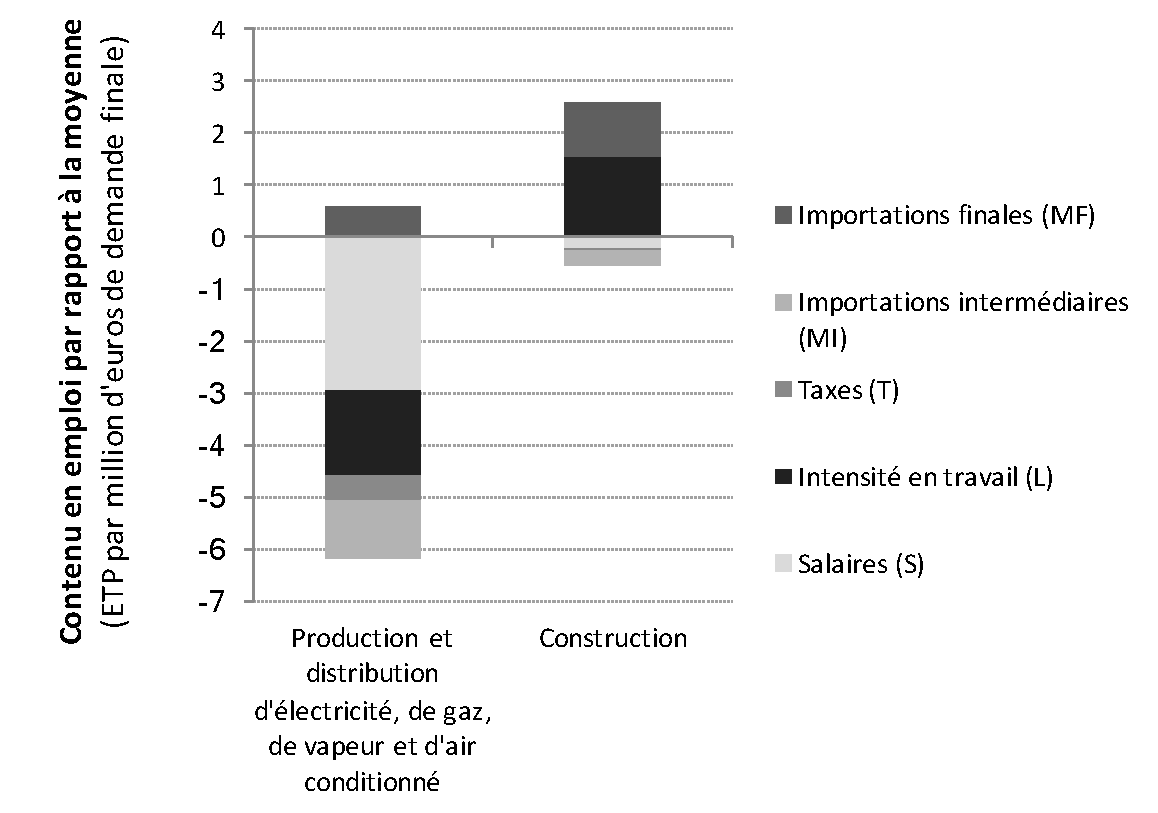
\includegraphics[width=12cm]{figures/comparaison1.pdf}
	\caption{Production et distribution d'électricité vs. Construction. \\ 
		Source : calculs des auteurs à partir de données Eurostat.}
	\label{fig:comparaison1}
	\captionsetup{justification=raggedright}
	\caption*{Lecture : ce graphique présente le contenu en ETP des deux branches F et D35 par rapport à la moyenne nationale, ainsi que la décomposition de cette différence. Allouer un million d'euros à la branche électricité-gaz génère 5,6 ETP de moins que la moyenne nationale. Cet effet négatif est essentiellement dû à des salaires élevés (- 3 ETP), à une faible part du travail dans la valeur ajoutée $L$ (- 1,6 ETP) et à des importations intermédiaires élevées (- 1,1 ETP). A l'inverse, la branche construction présente un contenu en emploi supérieur à la moyenne de 2 ETP par million d'euros de demande finale, principalement grâce à une forte part du travail dans la valeur ajoutée (+ 1,5 ETP) et un faible taux d'importations finales $MF$ (+ 1 ETP). 
	Réallouer un million d’euros de demande finale de la branche électricité-gaz vers la construction conduit à créer près de 7,6 ETP -- dont 3,1 ETP grâce à une plus grande part du travail dans la valeur ajoutée, et 1,3 ETP grâce à des importations plus faibles.}
\end{figure}

La figure \ref{fig:comparaison1} montre que la construction est moins intensive en émissions que la branche électrique et gazière. Et puisque l’isolation permet en plus de réduire les émissions directes des ménages (qui n’apparaissent donc pas dans la figure \ref{fig:ges_emploi}), le bilan total en GES est encore plus favorable à l’isolation. 
La figure \ref{fig:comparaison1} détaille les différences de contenu en emploi, et montre que la construction présente un contenu en emploi nettement plus important que la branche électricité. 
Cette différence provient essentiellement d'une plus forte part du travail dans la valeur ajoutée (à 42\%), des salaires plus faibles dans la branche construction (à 36\%) et d'importations plus faibles (à 17\%) dans la branche "Construction". Quant aux taxes et subventions, elles ne jouent qu’un rôle mineur (5\%). 
Une politique visant à promouvoir les économies d’énergies via l’isolation des bâtiments parait donc potentiellement génératrice d’emplois, et cela n’est dû qu’en partie à la faiblesse relative des salaires dans cette branche. 
Ces bilans en ETP ne tiennent pas compte des effets de friction temporaires, de l’inertie des migrations interbranches des employés \citep{Duhautois2005} ni de tous les ajustements sur le marché des biens et du travail. Mais ils fournissent une indication au premier ordre de l’effet sur l’emploi d’une réallocation de la demande finale.

\subsubsection{Deuxième exemple : réduire la consommation de carburant grâce aux  transports en commun}

Les transports en commun terrestres consomment moins de carburant et émettent moins de CO\textsubscript{2} par passager que les véhicules particuliers, mais qu’en est-il de leur contenu en emploi ? Une telle substitution implique une modification de la demande adressée à différentes branches, et les transports en commun ne sont pas distingués du fret routier et ferroviaire à ce niveau de désagrégation. 
Cependant, une comparaison entre les branches H49 « transports terrestres et transports par conduite » et C19 « cokéfaction et raffinage » (figure \ref{fig:comparaison2}) fournit un premier éclairage. Une moindre utilisation des véhicules particuliers va réduire l’activité dans le raffinage de pétrole. Et la réallocation d’un million d’euros d’une branche à l’autre permet de créer 12 ETP. Hors effet de salaires et de taxes (qui pénalisent la branche C19), la différence s’élève encore à 8 ETP.

\begin{figure}[!ht]
	\centering
	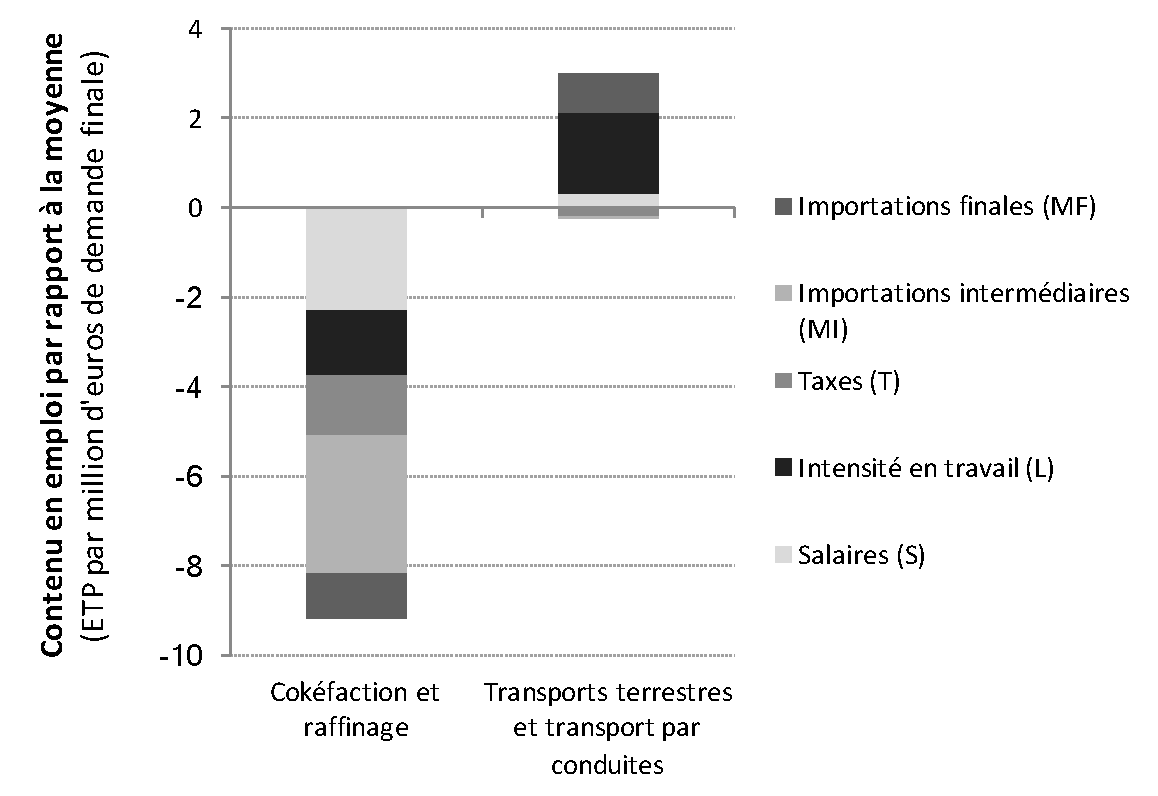
\includegraphics[width=12cm]{figures/comparaison2.pdf}
	\caption{Cokéfaction et raffinage vs. Transports terrestres. \\
		Source : calculs des auteurs à partir de données Eurostat.}
	\label{fig:comparaison2}
	\captionsetup{justification=raggedright}
	\caption*{Le faible contenu en emploi de la branche "Cokéfaction" par rapport à la moyenne s'explique essentiellement par de fortes importations intermédiaires (-3 ETP) et finales (- 1 ETP), ainsi que par de forts salaires (- 2,3 ETP) et la faible intensité en travail (-1,4 ETP). L'impact des taxes est ici marqué (-1,3 ETP). A l'inverse, la branche "Transports terrestres" présente un contenu en emploi supérieur à la moyenne, essentiellement grâce à un forte intensité en travail (+ 1,8 ETP) et de faibles importations finales (+ 0,9 ETP).}
\end{figure}

Cette comparaison ne prend pas en compte les effets dynamiques à plus long terme, par exemple la réduction de l’activité des producteurs d’automobiles. Mais elle fournit une explication des mécanismes de court terme. La décomposition peut également donner une intuition des mécanismes à l’œuvre dans les modèles macroéconomiques. Dans notre exemple, on peut s'attendre à un effet positif sur l'emploi provenant hausse de la production locale au détriment des importations et d'une plus forte demande de travail provenant de la part plus importante du travail dans le processus de production.


\section{Conclusion et discussion}

Nous calculons le contenu en emploi et le contenu en GES de 64 branches de l’économie française. 
Ces mesures sont utiles pour étudier des politiques publiques jouant sur la demande. 
Par exemple, améliorer l’efficacité énergétique dans le bâtiment diminue la demande d’énergie et augmente la demande des activités améliorant cette efficacité. Nos calculs fournissent une première approximation de cet effet.

Cependant, l’analyse agrégée que nous avons menée en distinguant 64 branches masque des disparités intra-branches. Prenons l’exemple de la production d’électricité : celle-présente un contenu en émissions de GES et en emploi très différents selon que l’électricité est produite à partir de charbon ou de sources renouvelables. 
Or la branche « production d’électricité et de gaz » du TES agrège ces différentes sources.

Pour obtenir des résultats plus fins, il est possible d’appliquer la même méthodologie à une branche en particulier, en détaillant des sous-branches. 
Par exemple, on pourrait distinguer les différentes filières de production d’électricité : photovoltaïque, éolien, nucléaire, gaz, charbon, etc. 
Une difficulté serait alors de reconstituer les données, car les agences de statistiques ne fournissent pas des données clés en main pour ce niveau de désagrégation. 
Pour chaque filière, il faudrait alors déterminer la production totale, le nombre d’emplois directs et une décomposition des consommations intermédiaires (donc de la chaîne de valeur) afin de déterminer le contenu en emploi. 
Il faudrait également estimer les émissions directes, et réutiliser la décomposition des consommations intermédiaires pour déterminer le contenu en GES (par exemple en se basant sur les données \citet{InNumeri2016} pour les emplois et ceux de \citet{Lehr2008} pour les consommations intermédiaires).

Par ailleurs, la réallocation d’un million d’euros de demande finale d’une branche vers une autre ne va pas générer un nombre d’emplois égal à la différence de leurs contenus en emploi. 
En effet, ce déplacement va entraîner d’autres effets et des ajustements sur les marchés du travail et des biens, qui ne sont pas pris en compte par notre approche comptable. 
Cette dernière ne cherche donc aucunement à se substituer aux autres analyses existantes, en particulier aux analyses d’équilibre général. Au contraire, ces deux approches sont complémentaires. D'ailleurs, dans le chapitre \ref{chap:mechanisms}, j'utilise des modèles d'équilibre général pour prolonger les réflexions menées dans ce chapitre.

Cependant, notre analyse descriptive peut fournir une indication quant au sens, positif ou négatif, des évolutions entrainées par l’évolution de la demande – tant sur l’emploi que sur les émissions de gaz à effet de serre. 
Cette évolution de la demande finale peut être générée par des mécanismes fiscaux incitatifs. 
Par exemple, taxer le carbone peut encourager l’utilisation de transports en commun. 
Il serait également possible d’inclure l’aspect intensif en travail pour définir les aides d’Etat et orienter les choix technologiques (par exemple l'isolation des logements est certainement plus intensive en travail que la capture et le stockage géologique du CO\textsubscript{2}). 
Enfin, une autre option consiste en un investissement direct de l’Etat, par exemple dans les transports en commun.

En outre, nos résultats concordent avec les analyses en équilibre général qui ont été menées en France lors du débat national sur la transition énergétique. Ils permettent de mieux comprendre les mécanismes entrant en jeu dans les modèles d’équilibre général et les phénomènes de double dividende environnement-emploi observés dans de nombreuses simulations menées à l’aide de ces modèles.

Nos résultats confirment qu’il est essentiel de comprendre la composition du contenu en emploi pour donner un sens à cette mesure. 
Ainsi, l’agriculture semble de prime abord présenter un contenu en emploi bien plus élevé que la moyenne de l’économie. Mais la présence de subventions explique la moitié de cette différence positive par rapport à moyenne, et ces subventions vont nécessiter des prélèvements grevant l’activité dans d'autres branches. 
La méthodologie que nous présentons permet de calculer un contenu en ETP hors effet des taxes et des subventions. En outre, identifier la part des différences de salaire dans les différences de contenu en emploi entre branches est utile pour juger de l’intérêt de certaines substitutions interbranches d’un point de vue social.

Enfin, nous montrons que de nombreuses branches fortement émettrices de gaz à effet de serre sont peu intensives en emploi. C’est notamment le cas des branches incluses dans l’EU ETS. Il semble donc qu’il puisse exister un potentiel pour réussir une transition énergétique qui réduise les émissions tout en favorisant les branches à fort contenu en emploi.



